\documentclass{beamer}
%\usetheme{default}    
\usetheme{Berkeley}    
\usecolortheme{crane}

\title{Consistency in the Cloud II}
\subtitle{Consistency v. Latency in Geo-Replicated Systems}
\author{Satabdi Aditya and Shannon Harwick}
\institute{University of Illinois at Chicago}
\titlegraphic{}
\date{\today}

\begin{document}


% --------------------------------------------------- Slide --0

\section{Li et al.} 

\begin{frame}
\frametitle{Paper 1: Li et al.}

\textbf{Title} Making Geo-Replicated Systems Fast as Possible,Consistent when necessary\newline
\textit{10th USENIX Symposium on Operating Systems Design and Implementation} \newline
Authors\newline
Date\newline

\end{frame}

% --------------------------------------------------- Slide --1

\begin{frame}
\frametitle{Motivation:}
\begin{enumerate}
\item To improve user-experience, services replicate  system state across geographical diverse sites.
\item Performance vs Consistency
\begin{itemize}
\item Amazon\'s Dynamo - eventual consistency where state temporarily diverge.
\item Yahoo PNUTS - avoids state divergence by requiring all operations that update the service state to be funneled through a primary site and thus incurring increased latency.
\end{itemize}
\end{enumerate}

\end{frame}


% --------------------------------------------------- Slide --2

\begin{frame}
\frametitle{Overview:}
\begin{enumerate}
\item RedBlue Consistency - Blue operations execute locally and are lazily replicated.Red operations are serialized with respect to each other and are immediately cross-site coordinated.
\item Conditions under which operations must be colored red or blue.
\item Decomposing operations into two components - a generator operation and a shadow operation.
\end{enumerate}

\end{frame}


% --------------------------------------------------- Slide --3

\begin{frame}
\frametitle{Properties of Geo-Replicated Systems}
\begin{enumerate}
\item Low latency - Operations should proceed after contacting a small number of users.
\item Causality - Monotonicity of user request within session and also preserving causality across clients
\item State Convergence - All replicas have executed the same set of operations
\item All operations should return a single value.
\item The system should provide a set of stable histories and support for general operations.
\item The system should preserve a set of invariants.
\item Eventual Propagation
\end{enumerate}
\end{frame}
% --------------------------------------------------- Slide --4

\begin{frame}
\frametitle{Related Work: Target end-to-end Properties}
\begin{figure}[t]
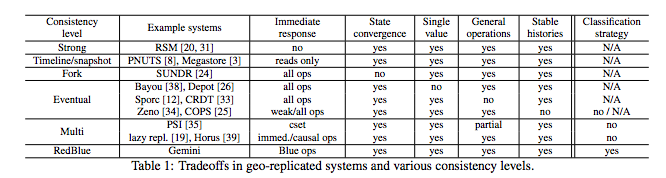
\includegraphics[width=10cm]{pic1.jpg}
\centering
\end{figure}
\end{frame}

% --------------------------------------------------- Slide --5

\begin{frame}
\frametitle{Related Work: Strong vs Weak Consistency}
\begin{enumerate}
\item
\end{enumerate}

\end{frame}


% --------------------------------------------------- Slide --6

\begin{frame}
\frametitle{Related Work: Other}
\begin{enumerate}
\item
\end{enumerate}

\end{frame}


% --------------------------------------------------- Slide --7

\begin{frame}
\frametitle{System Model}
\begin{enumerate}
\item
\end{enumerate}

\end{frame}

% --------------------------------------------------- Slide --8

\begin{frame}
\frametitle{RedBlue Consistency}
\begin{enumerate}
\item
\end{enumerate}

\end{frame}


% --------------------------------------------------- Slide --8

\begin{frame}
\frametitle{RedBlue Consistency - Definition}
\begin{enumerate}
\item
\end{enumerate}

\end{frame}

% --------------------------------------------------- Slide --8

\begin{frame}
\frametitle{State Convergence and RedBlue Bank}
\begin{enumerate}
\item
\end{enumerate}

\end{frame}

% --------------------------------------------------- Slide --9

\begin{frame}
\frametitle{Replicating side effects - Defining shadow operations}
\begin{enumerate}
\item
\end{enumerate}

\end{frame}

% --------------------------------------------------- Slide --10

\begin{frame}
\frametitle{Revisiting RedBlue consistency}
\begin{enumerate}
\item
\end{enumerate}

\end{frame}



%%% BEGIN SHANNON SECTION %%%
% --------------------------------------------------- Slide --

\section{Lloyd et al.} 

\begin{frame}
\frametitle{Paper 2: Lloyd et al.}

\textbf{Stronger Semantics for Low-Latency Geo-Replicated Storage} \newline
\textit{Proceedings of the 10th USENIX Symposium on Networked Systems Design and Implementation (NSDI’13)} \newline
Wyatt Lloyd, Michael J. Freedman, Michael Kaminsky, and David G. Andersen \newline
April 2013 \newline

\end{frame}

% --------------------------------------------------- Slide --
\begin{frame}
\frametitle{Main Idea}
\begin{itemize}

\pause \item Take slight hit in throughput to get stronger version of consistency
\pause \item Causal Consistency Instead of Eventual Consistency (causal is stronger)
\pause \item We require low latency
\pause \item Extend previous systems: Cassandra and COPS

\end{itemize}  
\end{frame}

% --------------------------------------------------- Slide --
\begin{frame}
\frametitle{Contributions}
\begin{itemize}
\pause \item Eiger
	\begin{itemize}
		\item Low Latency
		\item High throughput (slightly lower than Cassandra)
		\item Causal Consistency (rather than eventual as in Cassandra)
	\end{itemize}
\pause \item Read Only Algorithm
\pause \item Write Only Algorithm
\end{itemize}  
\end{frame}

% --------------------------------------------------- Slide --
\begin{frame}
\frametitle{Background}
\begin{itemize}
\pause \item Cassandra
	\begin{itemize}
		\item Eventual Consistency
	\end{itemize}
\pause \item COPS
\end{itemize}  
\end{frame}

% --------------------------------------------------- Slide --
\begin{frame}
\frametitle{Consistency - Causal versus Eventual}
\begin{itemize}
\pause \item p1	
\end{itemize}  
\end{frame}

% --------------------------------------------------- Slide --
\begin{frame}
\frametitle{Column Family Data Model}
\begin{itemize}
\pause \item p1 % Each \pause creates a new slide within the frame.
\pause \item p2
\pause \item p3
\end{itemize}  
\end{frame}



% --------------------------------------------------- Slide --
\begin{frame}
\frametitle{Eiger}
\begin{itemize}
\pause \item p1 % Each \pause creates a new slide within the frame.
\pause \item p2
\pause \item p3
\end{itemize}  
\end{frame}

% --------------------------------------------------- Slide --
\begin{frame}
\frametitle{Evaluation}
\begin{itemize}
\pause \item Versus Cassandra
		\begin{itemize}
			\item Within 7\% of throughput Using Facebook-like data
			\begin{itemize}
				\item Ops/sec
				\item Keys/sec
				\item Columns/sec
			\end{itemize}
		\end{itemize}
\pause \item Versus COPS
		\begin{itemize}	
			\item Both have low latency
			\item Eiger has slightly higher latency due to 2nd round indirection
			\item Only Eiger has write transactions
			\item Eiger has less overhead because it tracks only one-hop dependencies
		\end{itemize}
\end{itemize}  
\end{frame}

% --------------------------------------------------- Slide --
\begin{frame}
\frametitle{Follow Up Research}
\begin{itemize}
\pause \item Mahajan et al. showed that Causal Consistency strongest that guarantees low latency.
\end{itemize}  
\end{frame}

% --------------------------------------------------- Slide --
\begin{frame}
\frametitle{Ideas for Future Research}
\begin{itemize}
\pause \item p1 
\end{itemize}  
\end{frame}


% --------------------------------------------------- Slide --

\section{Bibliography} 

\begin{frame}
\frametitle{Bibliography}


%%% SHANNON'S REFERENCES
\begin{itemize}
\item \textbf{Stronger Semantics for Low-Latency Geo-Replicated Storage}, 
\textit{Proceedings of the 10th USENIX Symposium on Networked Systems Design and Implementation (NSDI’13)}, 
Wyatt Lloyd, Michael J. Freedman, Michael Kaminsky, and David G. Andersen, 
April 2013

\item \textbf{Out in the Open: The Abandoned Facebook Tech That Now Helps Power Apple}, 
\textit{www.wired.com}
, Klint Finley, Aug. 4, 2014

\item \textbf{A Short Primer on Causal Consistency}, 
\textit{;login: The Usenix Magazine Volume 38, Number 4}, 
Wyatt Lloyd, Michael J. Freedman, Michael Kaminsky, and David G. Andersen, , August 2013


\end{itemize}  
\end{frame}




\end{document} 